\documentclass[preview]{standalone}
\usepackage{header_problems}
\usepackage{header_template}
\begin{document}
\fontsize{12}{15}\selectfont

\Question{Getting Started}

\textbf{Read through this page carefully.} You may typeset your homework in latex or submit neatly handwritten/scanned solutions. Please start each question on a new page. Deliverables:

\begin{enumerate}
  \item Submit a PDF of your writeup, 
  %\textbf{with an appendix for your code}, 
  to assignment on Gradescope, ``<<title>> Write-Up". 
  %If there are graphs, include those graphs in the correct sections. Do not simply reference your appendix.
  %\item If there is code, submit all code needed to reproduce your results, ``<<title>> Code".
  %\item If there is a test set, submit your test set evaluation results, ``<<title>> Test Set".
\end{enumerate}

%After you've submitted your homework, watch out for the self-grade form.

\begin{Parts}

\Part Who else did you work with on this homework? In case of course events, just describe the group. How did you work on this homework? Any comments about the homework?

\vspace{15pt}
\framebox(465, 75){}

\Part Please copy the following statement and sign next to it. We just want to make it \textit{extra} clear so that no one inadvertently cheats.

\textit{I certify that all solutions are entirely in my words and that I have not looked at another student's solutions. I have credited all external sources in this write up.}

\vspace{15pt}
\framebox(465, 75){}

\end{Parts}

\pagebreak

This homework is due \textbf{Wednesday, December 5 at 10pm.}
\Question{Running Time of $k$-Nearest neighbor Search Methods}

The method of $k$-nearest neighbors is a very simple idea that forms a fundamental conceptual building block of machine learning, and plays a role in many ML algorithms. A classic example is the $k$-nearest
neighbor classifier, which is a non-parametric classifier that finds the $k$ closest examples in the training set to the test example, and then outputs the most common label among them as its prediction. Generating predictions using this classifier requires an algorithm to find the $k$ closest examples in a possibly large and high-dimensional dataset, which is known as the $k$-nearest neighbor search problem. More precisely, given a set of $n$ points, $\mathcal{D}=\{\vec{x}_{1}\ldots,\vec{x}_{n}\}\subseteq\mathbb{R}^{d}$ and a query point $\vec{z}\in\mathbb{R}^{d}$, the problem requires finding the $k$ points in $\mathcal{D}$ that are the closest to $\vec{z}$ in Euclidean distance.

This problem explores the computational complexity of nearest-neighbor methods to show how naive implementations perform very poorly as the dimensionality of the problem grows, but more sophisticated use of randomized techniques can do better. 

{\em Overall Hint: In this problem, reading later parts will help you know what you need to do in earlier parts in case you can't figure it out. So, read ahead before asking a question.}

\begin{Parts}
\Part First, we will try out a $k$-nearest neighbor classifier on the accessibility dataset collected earlier in the semester. Like in the previous homework, you should load, clean, and split the dataset into a test and train set, with 3000 datapoints in the test set. We will try two different classifiers: one which computes Euclidean distance in image feature space, and one which computes Euclidean distance on latitude and longitude. {\bf Plot test set accuracy curves of the two $k$-nearest neighbor classifiers for $k\in\{1, 5, 10, 15, 20, 25, 30\}$. } You may use scikit-learn methods.



\Part Now, let's consider the computational complexity of this algorithm. First, we consider the na\"{i}ve exhaustive search algorithm, which computes the distance between $\vec{z}$ and all points in $\mathcal{D}$ and then returns the $k$ points with the shortest distance. 
This algorithm first computes distances between the query and all points, then finds the $k$ shortest distances using quickselect\footnote{
Quickselect is a counterpart of quicksort that just picks the top $k$ in an unordered list. Instead of taking $O(n \log n)$ like quicksort on average, it takes $O(n)$. Look-up quickselect if you want, but in principle, you should be able to derive it if you understand the principle behind quicksort. Just realize that there is no point in recursively sorting things that for sure aren't going to be in the top $k$.}.
{\bf What is the (average case) time complexity of running the overall algorithm for a single query?} 



\Part Decades of research have focused on devising a way of preprocessing the data so that the $k$-nearest neighbors for each query can be found efficiently. ``Efficient'' means the time complexity of finding the $k$-nearest neighbors is lower than that of the na\"{i}ve exhaustive search algorithm -- meaning that the complexity must be \emph{sublinear} in $n$.

Many efficient algorithms for $k$-nearest neighbor search rely on a divide-and-conquer strategy known as space partitioning. The idea is to divide the feature space into cells and maintain a data structure that keeps track of the points that lie in each. Then, to find the $k$-nearest neighbors of a query, these algorithms look up the cell that contains the query and obtain the subset of points in $\mathcal{D}$ that lie in the cell and adjacent cells. Adjacent cells must be included in case the query point is in the corner of its cell. Then, exhaustive search is performed on this subset to find the $k$ points that are the closest to the query.

For simplicity, we'll consider the special case of $k = 1$ in the following questions, but note that the various algorithms we'll consider can be easily extended to the setting with arbitrary $k$. We first consider a simple partitioning scheme, where we place a Cartesian grid (a rectangular grid consisting of hypercubes) over the feature space.

\begin{figure}[h]
    \centering
    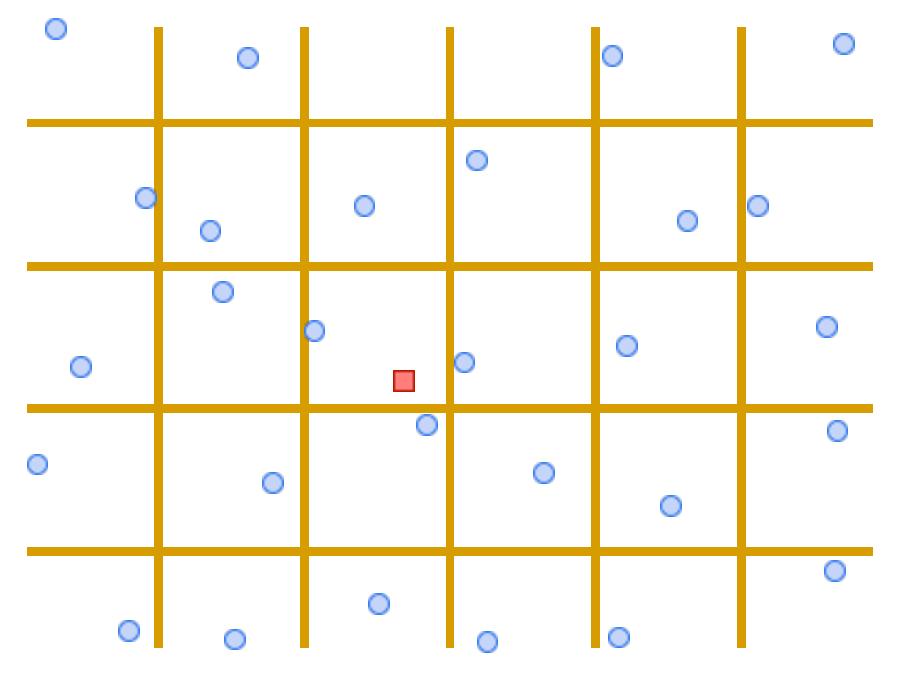
\includegraphics[width=0.4\textwidth]{src/problems/k_nn_running_time/partitioning}
    \caption{Illustration of the space partitioning scheme we consider. The data points are shown as blue circles and the query is shown as the red square. The cell boundaries are shown as gold lines.}
\end{figure}


{\bf How many cells need to be searched in total if the data points are one-dimensional? Two-dimensional? $d$-dimensional? If each cell contains one data point, what is the time complexity for finding the 1-nearest neighbor in terms of $d$, assuming accessing any cell takes constant time?}



\Part In low dimensions, the divide-and-conquer method provides a significant speedup over na\"{i}ve exhaustive search. However, in moderately high dimensions, its time complexity can grow large quickly. In the high dimensional case, we modify our divide-and-conquer algorithm to use the na\"{i}ve exhaustive search instead. 
This behavior arises in many settings, and is known as \emph{the curse of dimensionality}.
How do we overcome the curse of dimensionality? Since it arises from the need to search adjacent cells, what if we don't have cells at all?

Consider a new approach that simply projects all data points along a uniformly randomly chosen direction and keeps all projections of data points in a sorted list. To find the 1-nearest neighbor, the algorithm projects the query along the same direction used to project the data points and uses binary search to find the data point whose projection is closest to that of the query. Then it marches along the list to obtain $\tilde{k}$ points whose projections are the closest to the projection of the query. Finally, it performs exhaustive search over these points and returns the point that is the closest to the query. This is a simplified version of an algorithm known as Dynamic Continuous Indexing (DCI).

Because this algorithm is randomized (since it uses a randomly chosen direction), there is a non-zero probability that it returns the incorrect results. We are therefore interested in how many points we need to exhaustively search over to ensure the algorithm succeeds with high probability.

We first consider 
the probability that a data point that is originally far away appears closer to the query under projection than a data point that is originally close. 
Without loss of generality, we assume that the query is at the origin. 
Let $\vec{v}^{l}\in\mathbb{R}^{d}$ and $\vec{v}^{s}\in\mathbb{R}^{d}$ denote the far (long) and close (short) vectors respectively, and $\vec{u}\in S^{d-1}\subset\mathbb{R}^{d}$ is a vector drawn uniformly randomly on the unit sphere which serves as the random direction.
Then the event of interest is when $\{\left|\langle\vec{v}^{l},\vec{u}\rangle\right|\leq\left|\langle\vec{v}^{s}\vphantom{v^{l}},\vec{u}\rangle\right|\}$.

Assuming that $\vec{0}$, $\vec{v}^{l}$ and $\vec{v}^{s}$ are not collinear,\footnote{If $\vec{v}^{l}$ and $\vec{v}^{s}$ are collinear, random projection will essentially always be able to tell which is which so we don't bother to analyze that case. Understanding why will help you do this problem.} consider the plane spanned by $\vec{v}^{l}$ and $\vec{v}^{s}$, which we will denote as $P$.
For any vector $\vec{w}$, we use $\vec{w}^{\parallel}$ and $\vec{w}^{\perp}$ to denote the components of $\vec{w}$ in $P$ and $P^{\perp}$ such that $\vec{w}=\vec{w}^{\parallel}+\vec{w}^{\perp}$. 

{\bf If we use $\theta$ denote the angle of $\vec{u}^{\parallel}$ relative to $\vec{v}^{l}$, show that $\mathrm{Pr}\left(\left|\langle\vec{v}^{l},\vec{u}\rangle\right|\leq\left|\langle\vec{v}^{s}\vphantom{v^{l}},\vec{u}\rangle\right|\right) \leq \mathrm{Pr}\left(\left|\cos\theta\right| \leq \left\Vert \vec{v}^{s}\vphantom{v^{l}}\right\Vert _{2} / \left\Vert \vec{v}^{l}\right\Vert _{2}\right)$.}

\emph{Hint: For $\vec{w}\in\{\vec{v}^{s}\vphantom{v^{l}},\vec{v}^{l}\}$, because $\vec{w}^{\perp}=0$, $\langle\vec{w},\vec{u}\rangle=\langle\vec{w},\vec{u}^{\parallel}\rangle$. }

\begin{figure}[h]
    \centering
    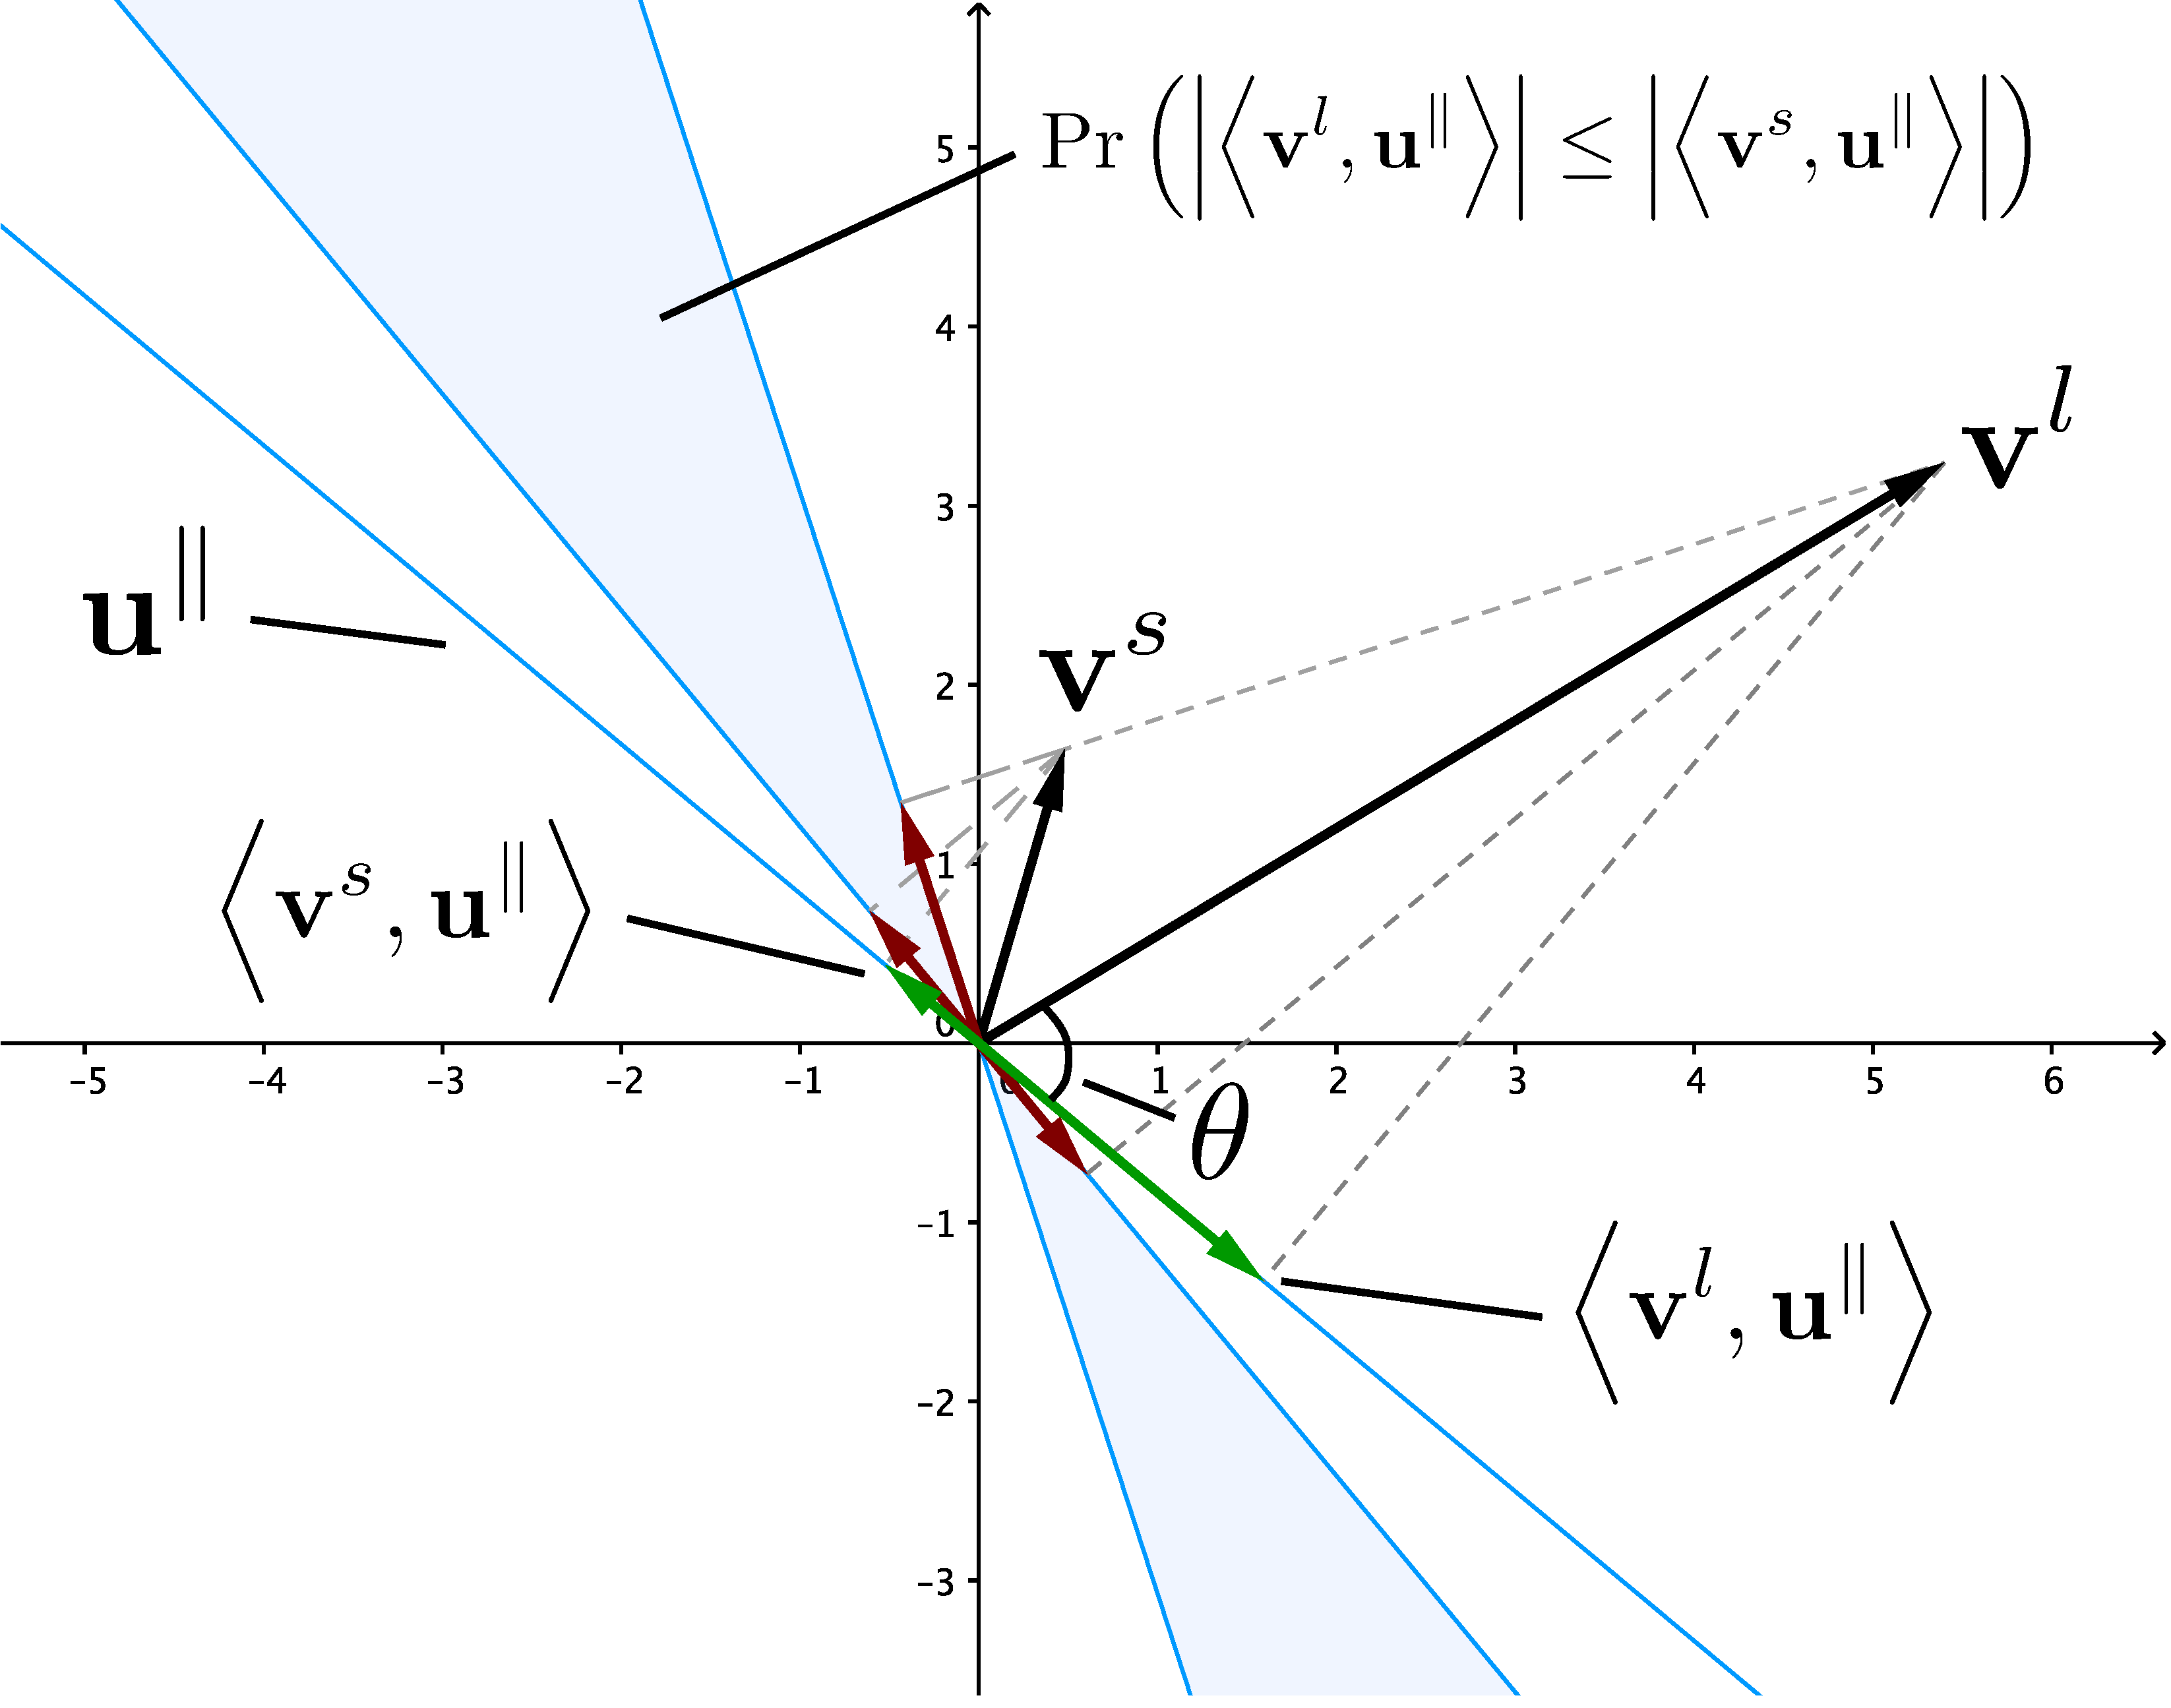
\includegraphics[width=0.4\textwidth]{src/problems/k_nn_running_time/dist_proj}
    \caption{Examples of ``good'' and ``bad'' projection directions. 
        The blue lines denote possible projection directions $\vec{u}^{\parallel}$. The isolated blue line represents a ``good'' projection direction, since the projection of $\vec{v}^{l}$ is longer than the projection of $\vec{v}^{s}$ (both shown in green), thereby preserving the relative order between $\vec{v}^{l}$ and $\vec{v}^{s}$ in terms of their lengths after projection. 
    Any projection direction within the shaded region is a ``bad'' projection direction, since the projection of $\vec{v}^{l}$ would not be longer than the projection of $\vec{v}^{s}$, thereby inverting the relative order between $\vec{v}^{l}$ and $\vec{v}^{s}$ after projection (shown in red). 
        }
\end{figure}



\Part

The algorithm would fail to return the correct $1$-nearest neighbor if more than $\tilde{k}-1$ points appear closer to the query than the $1$-nearest neighbor under projection. 

The following two statements will be useful:
\begin{itemize}

\item For any set of events $\left\{ E_{i}\right\} _{i=1}^{N}$, the probability that at least $m$ of them occur is at most $\frac{1}{m}\sum_{i=1}^{N}\mathrm{Pr}\left(E_{i}\right)$.\footnote{This is a generalization of the union bound; the statement reduces to the union bound when $k'=1$. (See this paper Ke Li and Jitendra Malik. Fast $k$-Nearest neighbor Search via Prioritized DCI. In \emph{Proceedings of the 34th International Conference on Machine Learning}, pages 2081--2090, 2017.)}
\item
$\mathrm{Pr}\left(\left|\cos\theta\right| \leq \left\Vert \vec{v}^{s}\vphantom{v^{l}}\right\Vert _{2} / \left\Vert \vec{v}^{l}\right\Vert _{2}\right) = 1-\frac{2}{\pi}\cos^{-1}\left(\left\Vert \vec{v}^{s}\vphantom{v^{l}}\right\Vert _{2}/\left\Vert \vec{v}^{l}\right\Vert _{2}\right)$. 
\end{itemize}



{\bf Using the first statement, derive an upper bound on the probability that the algorithm fails. Use $\vec{x}^{(i)}$ to denote the $i$th closest point to the query $\vec{z}$. Then use the second statement to simplify the expression.}



\Part


The following plots show the query time complexities of na\"{i}ve exhaustive search, space partitioning, and DCI as functions of $n$ and $d$. Curves of the same colour correspond to the same algorithm. (Assume that the failure probability of DCI is small) {\bf Which algorithm does each colour correspond to?}

\begin{center}
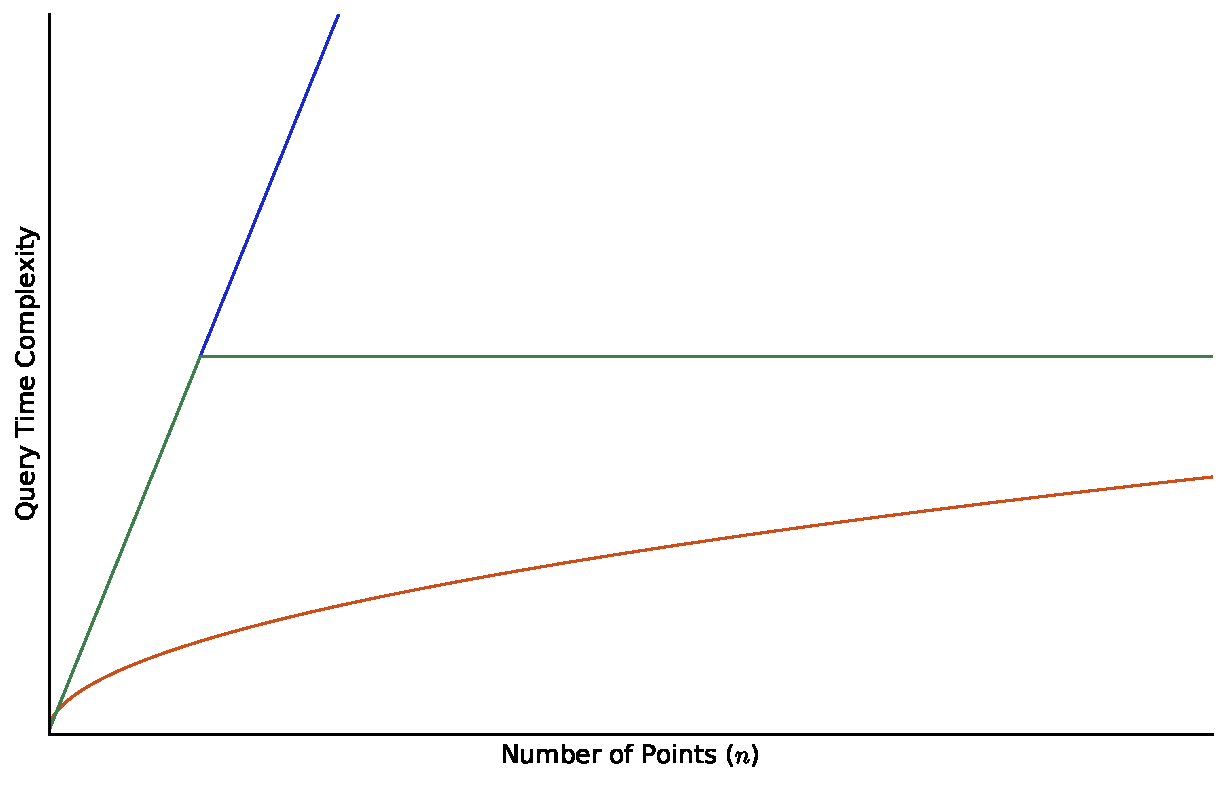
\includegraphics[width=0.4\textwidth]{src/problems/k_nn_running_time/dependence_on_n}
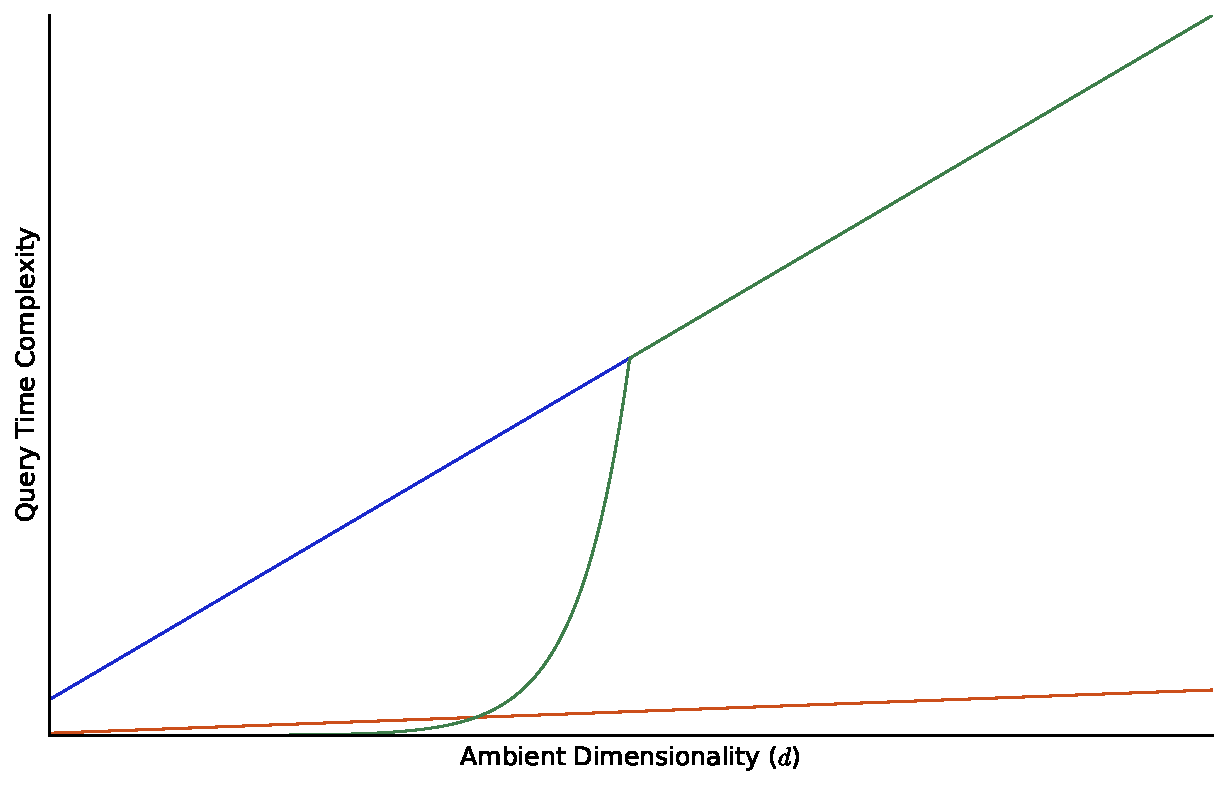
\includegraphics[width=0.4\textwidth]{src/problems/k_nn_running_time/dependence_on_d}
\end{center}




\Part  (Bonus)
We will now prove the second statement from (d).
{\bf Derive the range of $\theta$ such that $\left|\cos\theta\right| \leq \left\Vert \vec{v}^{s}\vphantom{v^{l}}\right\Vert _{2} / \left\Vert \vec{v}^{l}\right\Vert _{2}$ and show that \\
$\mathrm{Pr}\left(\left|\cos\theta\right| \leq \left\Vert \vec{v}^{s}\vphantom{v^{l}}\right\Vert _{2} / \left\Vert \vec{v}^{l}\right\Vert _{2}\right) = 1-\frac{2}{\pi}\cos^{-1}\left(\left\Vert \vec{v}^{s}\vphantom{v^{l}}\right\Vert _{2}/\left\Vert \vec{v}^{l}\right\Vert _{2}\right)$. }

\emph{Hint: Due to rotational invariance of a uniform distribution on the sphere, the angle between $\vec{u}^{\parallel}$ and any vector in $P$ is uniformly distributed.}

This part shows that the relative ordering of two data points is more likely to flip if their distances to the query are not very different.
Thus, the nearest neighbor search problem is harder if all data points are almost equidistant from the query.
The intrinsic hardness of the problem is characterized by the distribution of distances to the query.



\Part (Bonus) Notice that the failure probability of the randomized algorithm does not depend on dimensionality at all. It only depends on the distribution of distances from every point to the query, which measures the intrinsic hardness of the problem.

What's a typical distribution of distances? Natural data usually lies on a manifold, which is a generalization of Euclidean subspace that can be ``curved" (more concretely, there is a neighborhood around every point on the manifold that resembles a low-dimensional Euclidean space). For simplicity, we'll consider the case when the data is uniformly distributed on a $d'$-dimensional subspace, where $d'$ is much less than the ambient dimensionality $d$. Often, $d'$ is known as the intrinsic dimensionality. Then the number of points inside a ball of radius $r$ is roughly $cr^{d'}$ for some constant $c$. So, the number of points inside a ball of constant radius grows exponentially in $d'$.

Assume for all $r$ such that $cr^{d'}$ is an integer, the number of points inside a ball centerd at $\vec{z}$ of radius $r$ is exactly $cr^{d'}$. This is equivalent to saying $\Vert \vec{x}^{(cr^{d'})}-\vec{z}\Vert_{2}=r$ for any such $r$. (If we recall from the previous part, $\vec{x}^{(i)}$ denotes the $i$th closest point to $\vec{z}$. ) {\bf Show the quantity \\
$\sum_{i=2}^{n}\Vert \vec{x}^{(1)}-\vec{z}\Vert _{2}/\Vert \vec{x}^{(i)}-\vec{z}\Vert _{2}$ in this case is like $\sum_{i=2}^{n}\left(1/i\right)^{1/d'}$.}

\emph{Hint: to derive an expression for $\Vert \vec{x}^{(i)}-\vec{z}\Vert _{2}$ in terms of $i$, substitute $i$ for $cr^{d'}$ in the equality $\Vert \vec{x}^{(cr^{d'})}-\vec{z}\Vert_{2}=r$.}



\Part (Bonus) {\bf Show the quantity $\sum_{i=2}^{n}\left(1/i\right)^{1/d'}$ is less than $(n^{1-1/d'}-1)/\left(1-1/d'\right)$.}

\emph{Hint: use the fact that $\sum_{i=a}^{b}\phi(i)=\int_{a}^{b+1}\phi(\left\lfloor t\right\rfloor)dt$ for any function $\phi$ and $t-1<\left\lfloor t\right\rfloor $ for any $t$, where $\left\lfloor \cdot \right\rfloor$ denotes the floor operator.}



\Part (Bonus) {\bf Show the failure probability is at most $O(n^{1-1/d'}/\tilde{k})$ for $d' \geq 2$.}




\end{Parts}

\Question{Regularization and Risk Minimization}
\begin{Parts}
\Part
Let $\mat A$ be a $d \times n$  matrix. For any $\mu > 0$, show that $(\mat A\mat A^{\T} + \mu \mat I)^{-1}\mat A = \mat A(\mat A^{\T} \mat A + \mu \mat I)^{-1}$.

\Part Let $(\vec x_1, y_1), \cdots, (\vec x_n, y_n)$ be a sequence of data points. Each $y_i$ is a scalar and each $\vec x_i$ is a vector in $\R^d$. Let $\mat X = [\vec x_1, \dots, \vec x_n]^{\T}$ and $\vec y = [y_1, \dots, y_n]^{\T}$. Consider the $\textit{regularized}$ least squares problem. \\
  $$ \min_{\vec w \in \R^d} \;\lVert \mat X\vec w - \vec y\rVert_2^2 + \mu \lVert \vec w\rVert_2^2$$
Show that the optimum $\vec w_*$ is unique and can be written as the linear combination $\vec w_* = \sum_{i=1}^n \alpha_i \vec x_i$ for some scalars $\alpha_1,...,\alpha_n$. What are the coefficients $\alpha_i$?


\Part
More generally, consider the general regularized empirical risk minimization problem
  $$ \min_{\vec w \in \R^d} \; \frac{1}{n} \sum_{i=1}^n \text{loss}(\vec w^{\T} \vec x_i, y_i)  + \mu \lVert \vec w\rVert_2^2 $$
where the loss function is convex in the first argument. Prove that the optimal solution
has the form $\vec w_* = \sum_{i=1}^n \alpha_i \vec x_i$.
If the loss function is not convex, does the optimal solution have the form $\vec w_* = \sum_{i=1}^n \alpha_i \vec x_i$? Justify your answer.



\end{Parts}

\Question{Convergence Rate of Gradient Descent}

In homework 5 we showed that gradient descent converges for \textit{quadratic} functions, in this problem we will show that for any strongly convex function, gradient descent converges quickly. 
First, let us go through some definitions. It is possible to define a convex function $f$ as one where, for any $\vec x, \vec y \in \mathbb{R}^n$,
$$f(\vec x) + \nabla f(\vec x)^\top (\vec y-\vec x) \leq f(\vec y).$$
Geometrically, this means that if we start at $(\vec x, f(\vec x))$ and move along the gradient towards $(\vec y, f(\vec y))$, we end up ``below'' the actual value of $f(\vec y)$. We can extend this definition to a stronger one, saying that a function $f$ is $\alpha$-strongly convex if it satisfies
$$f(\vec x) + \nabla f(\vec x)^\top (\vec y-\vec x) + \frac{\alpha}{2} \|\vec x-\vec y\|^2 \leq f(\vec y).$$

Finally, a function $f$ is $\beta$-smooth if for any $\vec x, \vec y \in R^n$, one has 
$$\| \nabla f(\vec x) - \nabla f(\vec y) \| \leq \beta \|\vec x - \vec y\|.$$

\begin{Parts}

\Part \label{pt:smooth}
Let $\varphi$ be a $\beta$-smooth convex function.
Show that
\begin{align*}
(\nabla \varphi(\vec x) - \nabla \varphi(\vec y))^\top  (\vec x-\vec y) \geq \frac{1}{\beta} \| \nabla \varphi(\vec x) - \nabla \varphi(\vec y) \|^2
\end{align*}




\Part Let $f$ be $\beta$-smooth and $\alpha$-strongly convex. Show that $\varphi(\vec x) = f(\vec x) - \frac{\alpha}{2} \| \vec x \|^2$ is convex and $(\beta-\alpha)$-smooth.





\Part \label{pt:inequality}
Show that for all $\vec x,\vec y \in \mathbb{R}^n$, one has
\begin{align*}
(\nabla f(\vec x) - \nabla f(\vec y))^\top  (\vec x-\vec y) \geq \frac{\alpha \beta}{\beta + \alpha} \| \vec x - \vec y \|^2 + \frac{1}{\beta + \alpha} \| \nabla f(\vec x) - \nabla f(\vec y)\|^2
\end{align*}


\Part Let $f$ be $\beta$-smooth and $\alpha$-strongly convex, and denote $Q = \frac{\beta}{\alpha}$. Then show that gradient descent with fixed step size $\eta = \frac{2}{\alpha + \beta}$ satisfies
\begin{align*}
f(\vec x_t) - f(\vec x^*) \leq \frac{\beta}{2} \left( \frac{Q-1}{Q+1} \right)^{2(t-1)}\|\vec x_1 - \vec x^*\|^2
\end{align*}
\textbf{Hint:} By $\beta$-smoothness, you have
\begin{align*}
f(\vec x_t)-f(\vec x^*) \leq \frac{\beta}{2} \|\vec x_t-\vec x^*\|^2
\end{align*}






\end{Parts}


\end{document}
